\documentclass{article}
\usepackage{graphicx}
\usepackage{placeins}
\usepackage{float}
\usepackage[acronym,nomain]{glossaries}
\usepackage{titlesec}

\setcounter{secnumdepth}{4}


\makeglossaries

\begin{document}

\tableofcontents
\newpage
\printglossaries
\newpage

%%%%%%%%%%%%%%%%%%%%%%%%%%%%%%%%%%%%%%%%%%%%%%%%%%%%%%%%%%%%%%%%%%%%%%%%%%%%%%%%%%%%%%%%%
% Acronym definitions
\newacronym{sdn}{SDN}{Software Defined Network}
\newacronym{mno}{MNO}{Mobile Network Operators}
\newacronym{ngmn}{NGMN}{Next Generation Mobile Networks}
\newacronym{sil}{SIL}{Service Instance Layer}
\newacronym{nsil}{NSIL}{Network Service Instance Layer}
\newacronym{e2e}{E2E}{End to End}
\newacronym{e2e}{E2E}{End to End}
\newacronym{fh}{FH}{Fronthaul}
\newacronym{bh}{BH}{Backthaul}
\newacronym{cn}{CN}{Core Network}
\newacronym{vi}{VI}{Virtual Infrastructures}
\newacronym{IaaS}{IaaS}{Infrastructure-as-a-Service}
\newacronym{NS}{NS}{Network Services}
\newacronym{VNF}{VNF}{Virtual Network Functions}
\newacronym{MANO}{MANO}{Management and Orchestration}
\newacronym{NBI}{NBI}{Northbound Interface}
\newacronym{SBI}{SBI}{Southbound Interface}
\newacronym{MTA}{MTA}{Multi-Tenancy Application}
\newacronym{NF}{NF}{Network Functions}
\newacronym{CP}{CP}{Control Plane}
\newacronym{UP}{UP}{User Plane}
\newacronym{AN}{AN}{Access Network}
\newacronym{RAT}{RAT}{Radio Access Technology}


\section{Introduction}
Mobile networks are a key element of today's society, enabling communication, access
and information sharing. Moreover, traffic forecasts predict that the
demand for capacity will grow exponentially over the next years, mainly due to
video services. However, as cellular networks move from being voice-centric to
data-centric, operators' revenues are not able to keep pace with the predicted
increase in traffic volume. Such pressure on operators' return on investment has
pushed research efforts toward designing for 5G novel mobile network solutions
able to open the door for new revenue sources. In this context, the network
slicing paradigm has emerged as a key 5G disruptive technology addressing this
challenge.
Network slicing for 5G allows \gls{mno} to open
their physical network infrastructure platform to the concurrent deployment
of multiple logical self-contained networks, orchestrated in different ways according
to their specific service requirements; such network slices are then
(temporarily) owned by tenants. The availability of this vertical market multiplies
the monetization opportunities of the network infrastructure as new
players may come into play (e.g., automotive industry, e-health) and an higher
infrastructure capacity utilization can be achieved by admitting network slice
requests and exploiting multiplexing gains.
With network slicing for 5G networks, different services (e.g., automotive,
mobile broadband, or haptic Internet) can be provided by different network slice
instances. Each of these instances consists of a set of virtual network functions
that run on the same infrastructure with a tailored orchestration. In this way,
very heterogeneous requirements can be provided on the same infrastructure, as
different network slice instances can be orchestrated and configured separately
according to their specific requirements. Additionally, this is performed in a
cost-efficient manner as the different network slice tenants share the same
physical infrastructure.
A network slice is defined by \gls{ngmn} as “a set of network functions, and
resources to run these network functions, forming a complete instantiated
logical network to meet certain network characteristics required by the Service
Instance(s).”
According to NGMN, the concept of network slicing involves three layers,
namely, (i) service instance layer, (ii) network slice instance layer, and (iii)
resource layer. The \gls{sil} represents the end user and/or
business services provided by the operator or the third-party service providers,
which are supported by the \gls{nsil}. The NISL
is in turn supported by the resource layer, which may consist of the organic
resources such as compute, network, memory, storage, etc., or it may be more
comprehensive as being a network infrastructure, or it may be more complex
as network functions. Figure \ref{layers} depicts this concept where the resources at
the resource layer are dimensioned to create several sub network instances,
and network slice instances are formed that may use none, one, or multiple sub
network instances. 
\begin{figure}
\centering
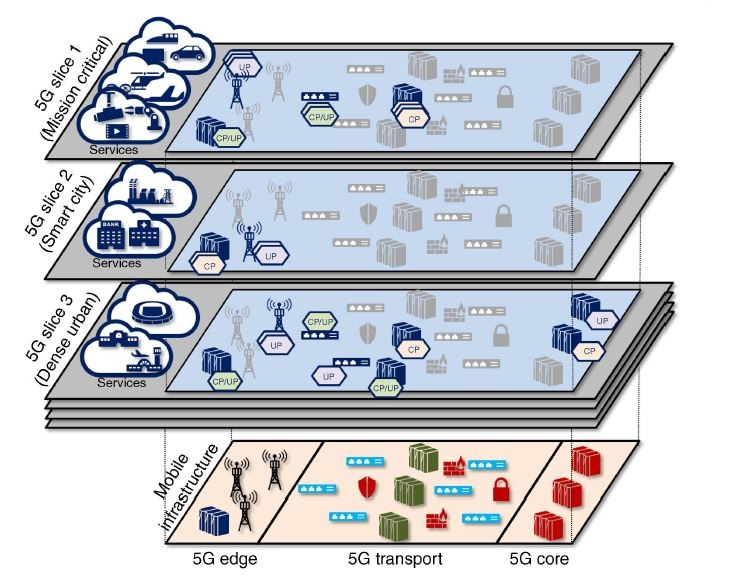
\includegraphics[scale=0.5]{pics/1.JPG}
\label{layers}
\caption{Example of network slicing in 5G.} 
\end{figure}
The end goal of network slicing in 5G mobile networks is to be able to realize
\gls{e2e} network slices starting from the mobile edge, continuing
through the mobile transport (\gls{fh} /\gls{bh}), and up until
the core network (CN). The allocation of a slice involves the selection of the
required functions, their constrained placement, the composition of the underlying infrastructure, and the allocation of the resources to fulfill the services' requirements, for example, bandwidth, latency, processing, resiliency.
We consider two main network slicing services that enable different degrees
of explicit control and are characterized by different levels of automation of the
mobile network slices management:
1) The provision of \gls{vi} under the control and operation
of different tenants-in line with an \gls{IaaS} model\footnote{form of cloud computing that provides virtualized computing resources over the internet},
that is, creation of a network slice instance.
2) The provision of tenant's owned \gls{NS}, that is, creation of a service instance.
In the former service, the deployment of a mobile network deals with the
allocation and deallocation of VIs. The logical entities within a VI encompassing
a set of compute and storage resources are interconnected by a virtual, logical
network (i.e., virtual nodes are interconnected by virtual links over the substrate
network). The Vis can be operated by the tenant via different \gls{sdn} control
models. In the latter, NS are instantiated directly over a shared infrastructure,
and as a set of interrelated \gls{VNF} connected through
one or more VNF forwarding graphs.
Multi-tenancy is an characteristic that can be applied to both
kinds of services, guaranteeing separation, isolation, and independence between
different slices coupled with the efficient sharing of the underlying resources
for both VI and NS concepts. In this context, a tenant is a logical entity owning and operating either one or more VIs or one or more network services. A tenant can be associated with an administrative entity (e.g., mobile virtual network operators) or
user of a given service (e.g., over-the-top service providers).


\newpage
\section{Architecture for Network Slicing}
The necessary architecture involves the aspects of modularization resource virtualization, virtual infrastructure, and network service management.
\begin{figure}[h]
\centering
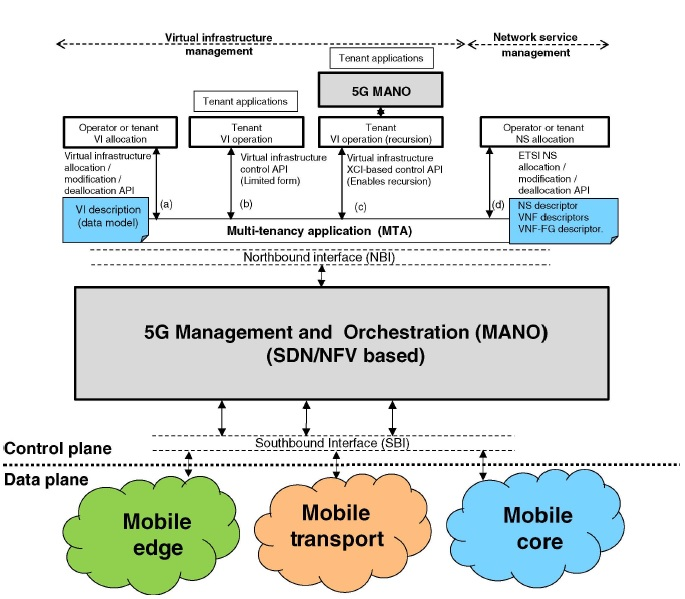
\includegraphics[scale=0.67]{pics/2.JPG}
\label{Arch}
\caption{Architecture for network slicing.} 
\end{figure}
The design proposed in Fig. \ref{Arch} follows the SDN principles of
(i) data and control plane fully decoupled, (ii) control logically centralized, and (iii) applications having an abstracted view of resources and states.
The data plane is the resource layer which includes mobile edge, mobile transport, and core. The infrastructure is composed of links, forwarding nodes (e.g., switches and routers), cloud nodes (e.g., data centers), and so on, comprising a set of network, computing, and storage resources.
The control plane is divided into two layers: an application layer at the top and the 5G \gls{MANO} platform below. The design
of the MANO is based on the ETSI management and network orchestration framework with integrated SDN-based control. The MANO
provides an abstracted view of available resources and states and control, and
management functions to an ecosystem of applications, via a \gls{NBI}. On the other hand, the MANO is connected to the data plane
elements via a \gls{SBI} to execute control and management
functions (e.g., OpenFlow, SNMP, OVSDB) on the actual hardware components.
With respect to the \gls{MTA}, it implements the
multi-tenancy support by coordinating and managing tenants access to a shared
infrastructure, performing resource isolation between instances assigned to
different tenants, and delivering multi-tenancy-related services, such as the
allocation and operation of VIs, by means of dedicated APIs in cooperation
with the data plane, enforcing this logical separation. As shown in Fig. \ref{Arch}
such APIs depend on the actual service: for the control of a VI or NS lifetime,
instantiation, modification, and deletion.

\subsection{Enablers and Design Principles}
Future 5G networks will be built on novel concepts that were not envisioned by the previous generation
network architectures. The revolution provided by the introduction of software-defined networking
and network function virtualization (NFV\footnote{NFV and VNF are often used interchangeably.}) opens the door to a
large list of possible applications recalling that the latter focuses primarily on optimization of the network services, instead the former to separate the control and forwarding plane for a centralized view of the network. The fundamental parts involved in the network slicing realization for the future 5G networks are now discussed.

\subsubsection{Modularization}
The evolution of mobile communication systems towards 5G was intentionally aiming at achieving
architecture flexibility, heterogeneous accesses and vertical business integration, leveraging on NFV and SDN. To enable the design of logical architectures tailored to
performance and functional requirements of different use cases, the principle of architecture
modularization and network function decomposition was proposed at the earliest 5G research
stages.\\ 
\gls{NF}s are functional blocks
that provide specific network capabilities to support and realize the particular service(s) demanded. Generally implemented
as software instances running on infrastructure
resources, NFs can be physical (a combination
of vendor-specific hardware and software, defin-
ing a traditional purpose-built physical appliance)
and/or virtualized (network function software is
decoupled from the hardware it runs on). In particular, conventionally monolithic network functions are proposed to be split into basic modules, both for the \gls{CP} and \gls{UP}, thus allowing the definition of different logical architectures via the interconnection of
different subsets of CP and UP NFs.
In the process of decomposing the NFs into basic modules, the distinction between NFs relating to
the \gls{AN} and core network emerged. To minimize the dependency of the 5G
core on the access (and vice versa), and achieve the definition of a convergent network\footnote{Network convergence is the efficient coexistence of telephone, video and data communication within a single network.}, providing
connectivity via a multitude of accesses not only including cellular radio, a different AN/CN functional split and an interface model are necessary.
Besides flexibility, the architecture modularization provides the essentials to support network
­slicing, as a network slice can be defined as an independent logical network shaped by the interconnection of a subset of NFs, composing both CP and UP, and which can be independently instantiated
and operated over physical or virtual infrastructure.




\subsubsection{Virtualization}
Virtualization is a key process for network slicing
as it enables effective resource sharing among
slices. Virtualization is the abstraction of resources
using appropriate techniques. Resource abstraction is the representation of a resource in terms of
attributes that match predefined selection criteria
while hiding or ignoring aspects which are irrelevant to such criteria, in an attempt to simplify the
use and management of that resource in some
useful way. The resources to be virtualized can
be physical or already virtualized, supporting a
recursive pattern with different abstraction layers.
Just as server virtualization makes virtual
machines (VMs) independent of the underlying
physical hardware, network virtualization enables
the creation of multiple isolated virtual networks that
are completely decoupled from the underlying physical network and can safely run on top of it.
The framework consists of\ three kinds of actors:\\
• Infrastructure provider (InP): owns and manages a given physical network and its constituent resources. Such resources, in the form of
WANs and/or data centers (DCs), are virtualized and then offered through programming
interfaces to a single or multiple tenants.\\
• Tenant: leases virtual resources from one or
more InPs in the form of a virtual network,
where the tenant can realize, manage, and
provide network services to its users. A network service is a composition of NFs, and it
is defined in terms of the individual NFs and
the mechanism used to connect them.\\
• End user: consumes (part of) the services
supplied by the tenant, without providing
them to other business actors.\\


%Through technologies like
%software-defined networking (SDN) and network
%functions virtualization (NFV), network softwarization can provide the programmability, flexibility,
%and modularity that is required to create multiple logical (virtual) networks, each tailored for a
%given use case, on top of a common network.
%These logical networks are referred to as network
%slices. The concept of separated virtual networks
%deployed over a single network is indeed not new
%(e.g., virtual private networks, VPNs); however,
%there are specificities that make network slices
%a novel concept. We define network slices as
%end-to-end (E2E) logical networks running on a
%common underlying (physical or virtual) network,
%mutually isolated, with independent control and
%management, which can be created on demand.
%Such self-contained networks must be flexible
%enough to simultaneously accommodate diverse
%business-driven use cases from multiple players on
%a common network infrastructure
%
%Future 5G networks will bring the concept of network programmability beyond what is now possible
%with SDN. While SDN splits routing and forwarding capabilities of a switch and reassigns the former
%to an SDN controller, this split between logic and agent should be performed for any NF, including
%the ones related to the CP. That is, the SDN principles are extended to all control and data layers as
%well as management functions usually deployed in mobile networks. 
%The following three categories can be identified: (i) networking control functions (e.g., mobility and
%session management, and potentially QoS/QoE control); (ii) connectivity control functions (mainly
%packet forwarding or SDN‐based packet forwarding); and (iii) wireless control functions (e.g., radio
%link adaptation and scheduling).
%There are many advantages of implementing selected wireless control functions in a way such that
%they are not bound anymore to specialized hardware, such as an LTE enhanced Node‐B (eNB), but
%rather become independent pieces of software. Network functionalities are then performed by a
%(virtualized) programmable and logically centralized controller that abstracts and, thus, homogenizes different network technologies. Such a controller will make network slices programmable
%by controlling the topology and functionality of the service chains as well as resource control inside
%the network slices. Further, this approach implies to have a unique control point for the network:
%By operating a small number of such controllers, network operators reduce the complexity of the
%network management and control.
%Dense wireless networks, as envisioned in 5G, will benefit from this extension of the SDN approach.
%The control of mobility support schemes and adaptation to dynamic radio characteristics, such as
%the ones used in a multiple radio access technology \gls{RAT} scenario, are performed by the controller
%that can employ especially tailored algorithms per network slice they are deployed in. Moreover, if
%needed, VNFs)can be deployed closely to the users (e.g., in a network slice supporting
%vehicular URLLC) reducing their experienced latency.

\subsubsection{Orchestration}
Orchestration is also a key process for network
slicing. In its general sense, orchestration can be
defined as the art of both bringing together and coordinating disparate things into a coherent whole.
In a slicing environment, where the players involved
are so diverse, an orchestrator is needed to coordinate seemingly disparate network processes for
creating, managing, and delivering services.
According to the ONF,
orchestration is defined as the continuing process of
selecting resources to fulfill client service demands
in an optimal manner. The idea of optimal refers
to the optimization policy that governs orchestrator behavior, which is expected to meet all the specific policies and service level agreements (SLAs)
associated with clients (e.g., tenants or end users)
that request services. The term continuing means
that available resources, service demands, and optimization criteria may change in time. Interestingly,
orchestration is also referred to as the defining
characteristic of an SDN controller. Note that client
is a term used in the SDN context.
The ONF states that the orchestrator functions
include client-specific service demand validation,
resource configuration, and event notification.
However, in network slicing, orchestration cannot be performed by a single centralized entity,
not only because of the complexity and broad
scope of orchestration tasks, but also because it
is necessary to preserve management independence and support the possibility of recursion. In
our view, a framework in which each virtualization
actor has an entity performing orchestration functions seems more suitable to satisfy the
above requirements. The entities should exchange
information and delegate functionalities between
them to ensure that the services delivered at a
certain abstraction layer satisfy the required performance levels with optimal resource utilization.
\paragraph{Isolation}
Strong isolation is a major requirement that must
be satisfied to operate parallel slices on a common shared underlying substrate. The isolation
must be understood in terms of:\\
• Performance: Each slice is defined to meet particular service requirements, usually expressed in the
form of key performance indicators (KPIs). Perfor-
mance isolation is an E2E issue, and has to ensure
that service-specific performance requirements are
always met on each slice, regardless of the congestion and performance levels of other slices.\\
• Security and privacy: Attacks or faults occurring in one slice must not have an impact on
other slices. Moreover, each slice must have
independent security functions that prevent unauthorized entities to have read or write access to
slice-specific configuration/management/accounting information, and be able to record any of
these attempts, whether authorized or not.\\
• Management: Each slice must be independently managed as a separate network.
To achieve isolation, a set of appropriate, consistent policies and mechanisms have to be defined
at each virtualization level, following the recursion
principle introduced earlier. The policies contain lists of rules that describe how different manageable entities must be properly isolated, without delving into how this can be achieved.
To fully realize the
required isolation level, the interplay of both virtualization and orchestration is needed.




\subsubsection{SDN}
The SDN architecture comprises an intermediate control plane that dynamically configures and abstracts the underlying
forwarding plane resources so as to deliver tailored services to clients located in the application plane. This is
well aligned with the requirements of 5G network
slicing, which needs to satisfy a wide range of service demands. Thus, the SDN architecture is an appropriate
tool for supporting the key principles of slicing.\\
The major SDN components are resources and controllers. For
SDN, a resource is anything that can be utilized to
provide services in response to client requests. This
includes infrastructure resources\footnote{Heterogeneous hardware and necessary software for hosting and connecting NFs. They include computing hardware,
storage capacity, networking resources (e.g., links
and switching/routing devices enabling network
connectivity), and physical assets for radio access.
} and NFs, but also
network services, in application of the recursion
principle described earlier. A controller is a logically centralized entity instantiated in the control
plane which operates SDN resources at runtime
to deliver services in an optimal way. Therefore,
it mediates between clients and resources, acting simultaneously as server and client via client
and server contexts, respectively. Both contexts
are conceptual components of an SDN controller
enabling the server-client relationships:\\
• Client context: Represents all the information the
controller needs to support and communicate with
a given client. It comprises a Resource Group and
a Client support function. The Resource Group contains an abstract, customized view of all the resources that the controller, through one of its northbound
interfaces, offers to the client, in order to deliver
on its service demands and facilitate its interaction
with the controller. Client support contains all that
is necessary to support client operations, including
policies on what the client is allowed to see and do and service-related information to map actions
between the client and the controller.\\
• Server context: Represents all the information the controller needs to interact with a set of
underlying resources, assembled in a Resource
Group, through one of its southbound interfaces.
The process of transforming the set of
Resource Groups accessed through server contexts to those defined in separate client contexts
is not straightforward, and it requires the SDN
controller to perform virtualization and orchestration functions.
When performing the virtualization function, the
SDN controller carries out the abstraction and the
aggregation/partitioning of the underlying resources. Thanks to virtualization, each client context provides a specific Resource Group that can be used by the client associated with that context to realize
its service(s). Through orchestration, the SDN controller optimally dispatches the selected resources
to such separate Resource Groups. The interplay
of both controller functions enables the fulfillment
of the diverging service demands from all clients
while preserving the isolation among them.
The SDN architecture also includes an administrator. Its tasks consist of instantiating and configuring the entire controller, including the creation
of both server and client contexts and the installation of their associated policies.
The SDN architecture naturally supports slicing, as the client context provides the complete abstract set of resources
(as a Resource Group) and the supporting control
logic that constitute a slice, including the complete
collection of related client service attributes.
Another key functional aspect that makes SDN
architecture ideal to embrace 5G slicing is recursion. Because of the different abstraction layers
that the recursion principle enables, the SDN
control plane can involve multiple hierarchically
arranged controllers that extend the client-server
relationships at several levels. According to
these premises, it is evident that SDN can support a
recursive composition of slices. This implies that
the resources (i.e., Resource Group) a given controller delivers to one of its clients in the form of a
dedicated slice (i.e., client context) can, in turn, be
virtualized and orchestrated by such a client in the
case of being an SDN controller. In this way, the new
controller can utilize the resource(s) it accesses via
its server context(s) to define, scale, and deliver
new resources (and hence new slices) to its own
clients, which might also be SDN controllers.


\subsubsection{VNF}
Although the SDN architecture described above
gives a comprehensive view of the control plane
functionalities enabling slicing, it lacks capabilities
that are vital to efficiently manage the life cycle of
network slices and its constituent resources. In this
respect, the NFV architecture is ideal to play
this role, as it manages the infrastructure resources
and orchestrates the allocation of such resources
needed to realize VNFs and network services.
In this respect, the NFV architecture is ideal to play
this role, as it manages the infrastructure resources
and orchestrates the allocation of such resources
needed to realize VNFs and network services.
To benefit from the management and orchestration functionalities of NFV, appropriate cooperation between SDN and NFV is required.
However, embracing SDN and NFV architectures
into a common reference framework is not an
easy task. ETSI presents a framework
to integrate SDN within the reference NFV architecture. This framework incorporates two SDN
controllers, one logically placed at the tenant and
another at the InP level. The NFV architecture comprises the following
entities:\\
• Network Functions Virtualization Infrastructure (NFVI): A collection of resources used to
host and connect the VNFs. While the broad
scope of SDN makes resource a generic concept,
the current resource definition in the NFV framework comprises only the infrastructure resources.\\
• VNFs: Software-based implementations of NFs
that run over the NFVI.\\
• Management and Orchestration (MANO):
Performs all the virtualization-specific management, coordination, and automation tasks in the
NFV architecture. The MANO framework
comprises three functional blocks:\\
• • Virtualized infrastructure manager (VIM):
responsible for controlling and managing the
NFVI resources.\\
• • VNF manager (VNFM): performs configuration and life cycle management of the
VNF(s) on its domain.\\
• • Orchestrator: According to ETSI, it has two
set of functions performed by the Resource
Orchestrator (RO) and Network Service
Orchestrator (NSO), respectively. The RO
orchestrates the NFVI resources across
(potentially different) VIMs. The NSO performs the life cycle management of network
services using the capabilities provided by the
RO and the (potentially different) VNFMs.\\
• Network Management System (NMS): Framework performing the general network management tasks. Although its functions are orthogonal
to those defined in MANO, NMS is expected to
interact with MANO entities by means of a clear
separation of roles. NMS comprises:\\
• • Element management (EM): anchor point
responsible for the fault, configuration,
accounting, performance, and security
(FCAPS) of a VNF.\\
• • Operation/business support system (OSS/
BSS): a collection of systems and manage-
ment applications that network service providers use to provision and operate their network
services. In terms of the roles we considered
earlier, tenants would run these applications.
The ETSI proposal includes two SDN controllers
in the architecture. Each controller centralizes
the control plane functionalities and provides an
abstract view of all the connectivity-related components it manages. These controllers are:\\
• Infrastructure SDN controller (IC): Sets up
and manages the underlying networking resources to provide the required connectivity for communicating the VNFs.
Managed by the VIM, this controller may change
infrastructure behavior on demand according to
VIM specifications adapted from tenant requests.\\
• Tenant SDN controller (TC): instantiated in
the tenant domain as one of the VNFs or as
part of the NMS, this second controller dynamically manages the pertinent VNFs used to realize
the tenant’s network service(s). These VNFs are
the underlying forwarding plane resources of the
TC. The operation and management tasks that the
TC carries out are triggered by the applications
running on top of it (e.g., the OSS).\\
Both controllers manage and control their
underlying resources via programmable southbound interfaces, implementing protocols like
OpenFlow, NETCONF, and I2RS. However, each
controller provides a different level of abstraction. While the IC provides an underlay to support
the deployment and connectivity of VNFs, the
TC provides an overlay comprising tenant VNFs
that, properly composed, define the network service(s) such a tenant independently manages on
its slice(s). These different resource views each
controller offers through its interfaces have repercussions on the way they operate. On one side,
the IC is not aware of the number of slices that utilize the VNFs it connects, nor the tenant(s) which
operate(s) such slices. On the other side, for the
TC the network is abstracted in terms of VNFs,
without notions of how those VNFs are physically
deployed. Despite their different abstraction levels,
both controllers have to coordinate and synchronize their actions. Note that the service and
tenant concept mentioned here can be extended
to higher abstraction layers by simply applying the
recursion principle.
\begin{figure}[h]
\centering
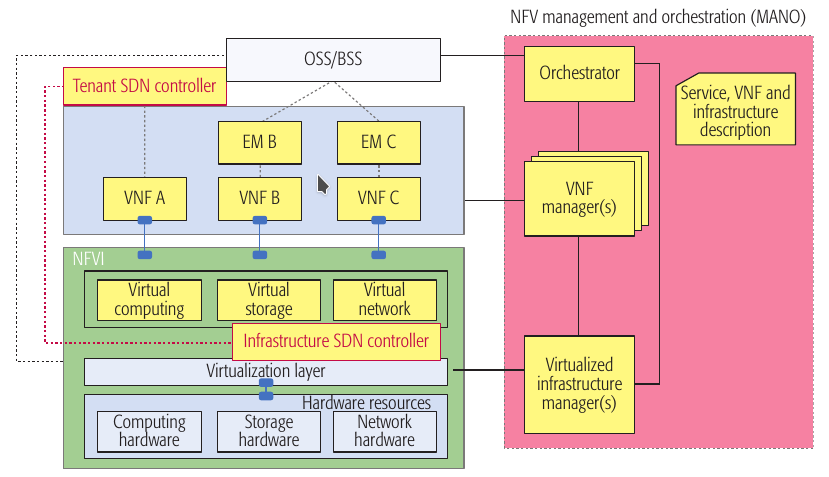
\includegraphics[scale=0.6]{pics/integral.png} 
\label{integral}
\caption{Integrating SDN controllers into the reference NFV architectural framework.}
\end{figure}



\newpage
\section{Network slicing} %da revisionare
In order to create tenant‐ or service‐specific networks, NGMN has proposed the concept of net-
work slicing [1], as detailed in Chapter 8. While legacy systems host multiple telecommunication
services, such as mobile broadband, voice, SMS, etc., on the same mobile network architecture, for
instance composed of Long Term Evolution (LTE) radio access and the Evolved Packet Core (EPC),
future 5G networks should also support shared or dedicated logical architectures customized to the
respective telco or vertical services, such as enhanced mobile broadband (eMBB), vehicular com-
munications, ultra‐reliable low‐latency communications (URLLC), and massive machine‐type com-
munications (mMTC), as introduced in Section 2.2. These services need very different KPIs that are
hard to be fulfilled by legacy systems, as they are characterized by monolithic network elements that
have tightly coupled hardware, software, and functionality. In contrast, future architecture leverages the decoupling of software‐based network functions from the underlying infrastructure resources by
means of utilizing different resource abstraction technologies.
Furthermore, as explained in the previous paragraph, modularization will play a fundamental role.
For instance, well‐known resource sharing technologies such as multiplexing and multitasking, e.g.,
wavelength division multiplexing (WDM) or radio scheduling, can be advantageously complemented
by softwarization techniques such as NFV and SDN. Multitasking and multiplexing allow sharing
physical infrastructure that is not virtualized. NFV and SDN allow different tenants to share the
same general‐purpose hardware, such as commercial off‐the‐shelf (COTS) servers. In combination,
these technologies allow building fully decoupled E2E networks on top of a common, shared infra-
structure. Consequently, multiplexing will not happen on the network level anymore, but on the
infrastructure level, as depicted in Figure 5‐1, yielding better quality of service (QoS) or quality of
experience (QoE) for the subscriber (as different slices will have tailored orchestration for a given
service) as well as improved levels of network operability for the mobile service provider or mobile
network operator.
In principle, a network slice is a logical network that provides specific network capabilities and
network characteristics and comprises NFs, computing and networking resources to meet the
­performance requirements of the tenants, for instance verticals. This comprises both radio access
network (RAN) and CN NFs and, depending on the degree of freedom that a tenant may have, also
the management and orchestration (MANO) components. A network slice may be dedicated to a
specific tenant or partially shared by several tenants that have the same performance requirements
but ­different security or policy settings. The decoupling between the virtualized and the physical
­infrastructure allows for the efficient scaling in, out, up or down of the slices, hence suggesting the
economic viability of this approach that can adapt the used resources on demand.
Network slices are created mostly with a business purpose: Following the 5G vertical markets para-
\begin{figure}[h]
\centering
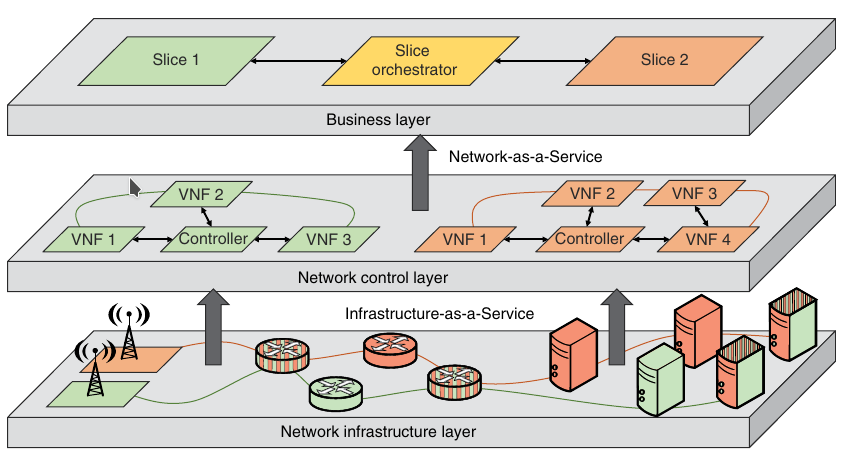
\includegraphics[scale=0.6]{pics/slice.png}
\label{slice}
\caption{An example of a network‐sliced architecture.} 
\end{figure}
5G atom. The 5G use cases are in the center. The layers , from the center out,
represent the requirements of the 5G use cases , the concepts that will allow network
operators to satisfy the requirements , the technologies that enable the implementation of
the concepts , and the novelties, that is, technologies that can be easily implemented due
to softwarization and virtualization techniques.
\begin{figure}[h]
\centering
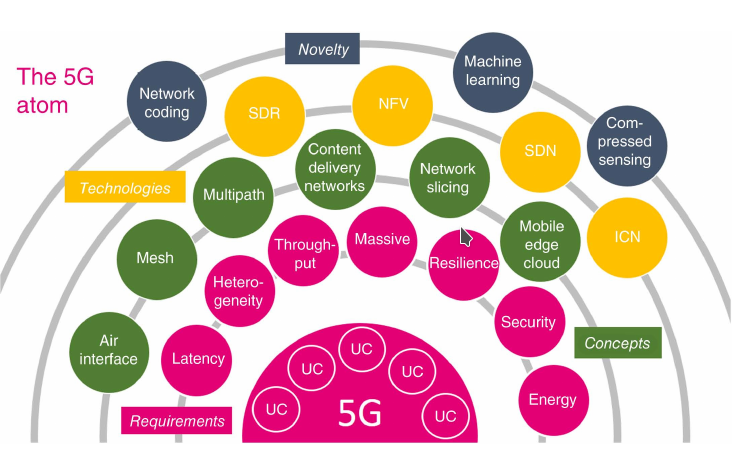
\includegraphics[scale=0.5]{pics/5g_atom.png} 
\label{atom}
\caption{5G atom rappresentation.}
\end{figure}


\subsection{Services}
\subsection{Example}
\subsection{Actual realizations}
bbbbb


\newpage
\nocite*
\bibliographystyle{plain}
\bibliography{biblist}

\end{document}